\documentclass{article}
\usepackage[]{url}
\usepackage{graphicx}
\usepackage{hyperref}
\usepackage{mathtools}
\usepackage{tikz}

\begin{document}
\title{Simulation of two interacting squirmers}
\author{Robin and Justine\\
\\
Supervisors: Van Landeghem Céline, Giraldi Laetitia,\\ Prud'Homme Christophe}
\date{May, 2024}
\maketitle

\tableofcontents

\section{Context}
Our project is part of the ANR project NEMO, Control of Magnetic Micro-swimmers in Complex and Confined Environments.
This projects aims to develop numerical methods for driving micro-robots composed of magnetic heads and flexible tails imitating spermatozoa, referred to as $Magnetozoon$.\cite{Nemov10}\\
The $Magnetozoon$ behavior is controlled by a magnetic field which produces a torque on the magnetic head leading to the motion of the tail.
This tail motion pushes the fluid surrounding the robot causing deformations and displacements of the robots.
Currently, a team of researchers is developing numerical methods to control a micro-swimmer in the arteries
of the human body. Ultimately, the goal of these robots is to treat cancer cells. \\
In this project, we study the interaction between squirmers. The squirmer is a model for a spherical microswimmer swimming in Stokes flow. \cite{Wikipedia}
A Stokes flow is a type of fluid flow where advective inertial forces are small compared with viscous forces.
The Squirmer model simulates bacteria with cilia by imposing boundary conditions.


\vspace{0.5cm}
\section{Objectives and Roadmap}
Our goal is to model the dynamics of two interacting squirmers, influenced by hydrodynamic \cite{Brumley} and collision forces.\\
We will start by reformulating the formulas of all present forces and torques.\cite{Brumley}\cite{Lauga}\\
In addition we will implement this model to realize numerical experiments. The aim of these experiments is: 
\begin{itemize}
    \item To Investigate the effects of varying the distance between the squirmers to observe
    potential modifications in their behaviors.
    \item To explore the impact of altering the parameter $\beta$, which defines the
    type of squirmers (pusher, puller, neutral swimmer), on their interactions.
    \item To conduct a comparative analysis of the interaction between a squirming micro-robot and a 
    boundary of the fluid domain. This analysis will involve varying the initial angle of the micro-robot, the distance between the swimmer and the wall, as well as the parameter $\beta$, 
    to comprehensively understand their influence on the system dynamics.
\end{itemize}

The original Roadmap of our project is given by:
\begin{center}
    \href{https://github.com/orgs/master-csmi/projects/23/views/2}{Roadmap}
    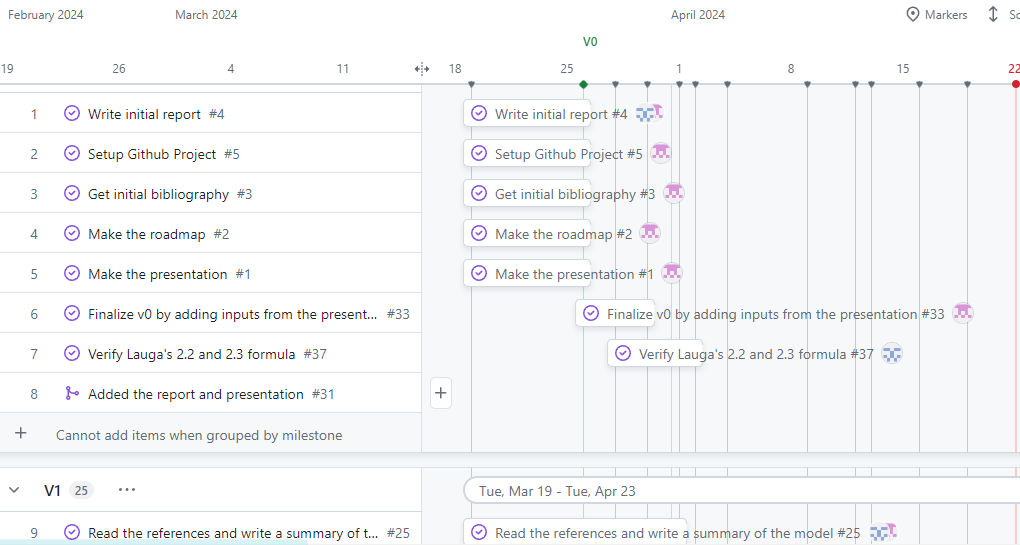
\includegraphics[width=1.2\textwidth]{Presentation/V0/images/roadmapV0_1.png}
    \vspace{1em} % Ajoute un espace vertical
    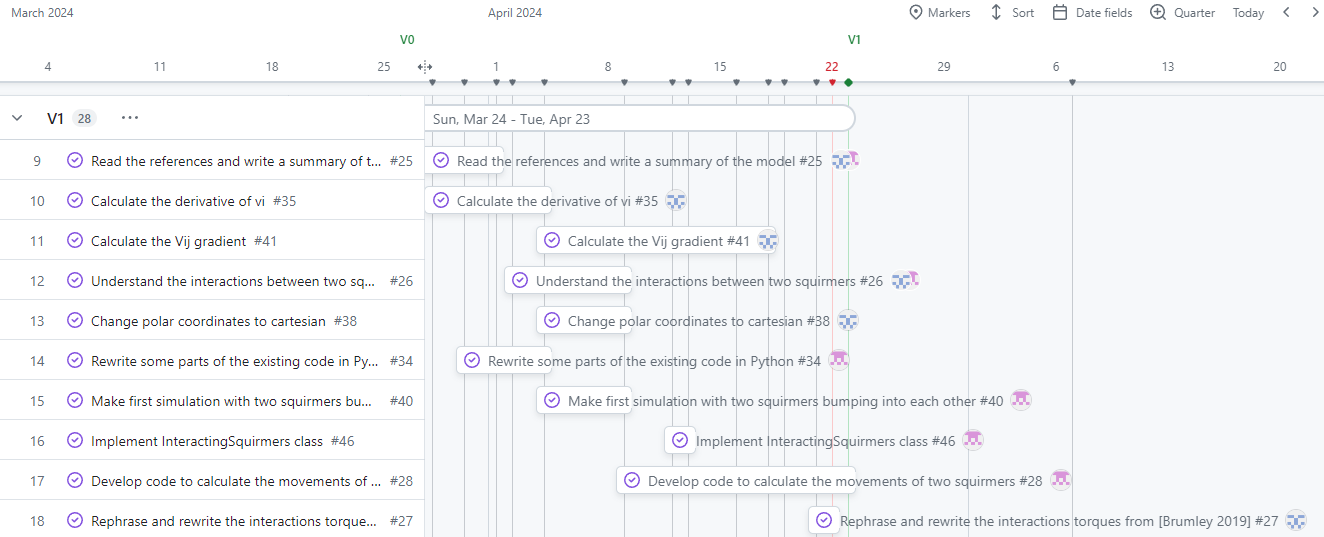
\includegraphics[width=1.2\textwidth]{Presentation/V0/images/roadmapV1_1.png}
    \vspace{1em} % Ajoute un espace vertical
    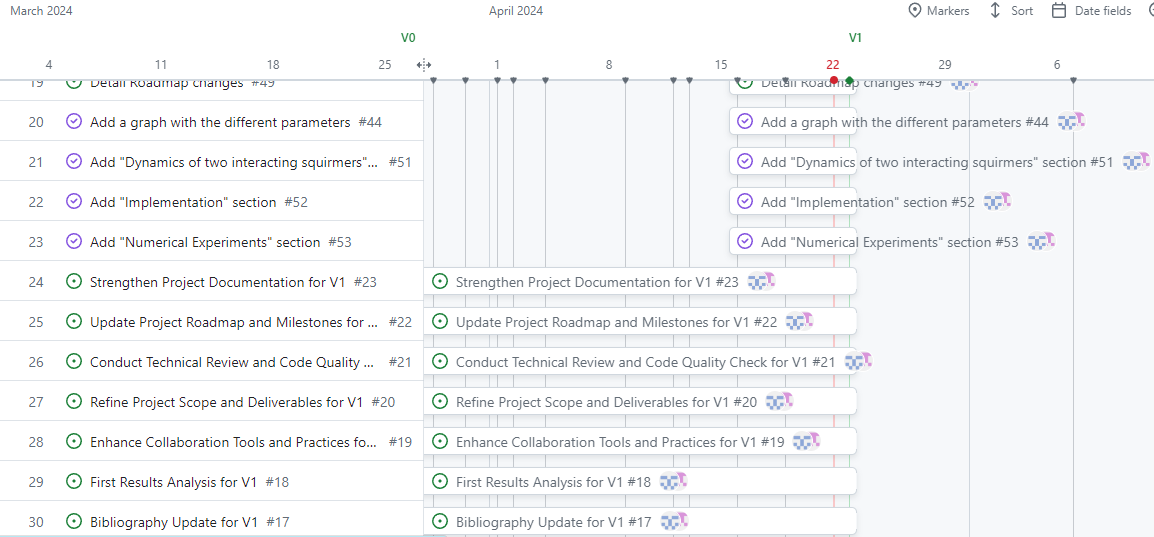
\includegraphics[width=1.2\textwidth]{Presentation/V0/images/roadmapV1_2.png}
\end{center}


\newpage
\section{Squirmer model}
\begin{center}
    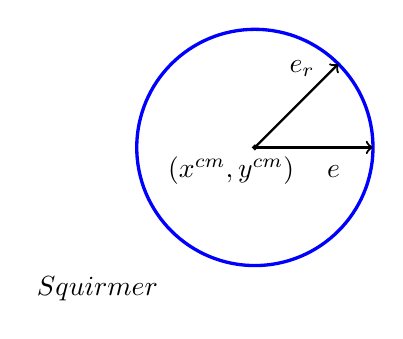
\begin{tikzpicture}
    
    \draw[color=blue, very thick](2.5,2.5) circle (1.5);
    
    \draw[color=black, very thick](2.5,2.5) circle (0.01);
    
    \node  at (2.5-0.3,2.5-0.3) {{$(x^{cm},y^{cm})$}};
    
    \node  at (0.5,0.7) {{$Squirmer$}};
    
    \draw[thick, ->] (2.5,2.5) -- (4,2.5);
    \node  at (3.5,2.2) {{$e$}};
 
    \pgfmathsetmacro{\xcoord}{2.5 + 1.5*cos(45)}
     \pgfmathsetmacro{\ycoord}{2.5 + 1.5*sin(45)}
     \draw[thick, ->] (2.5,2.5) -- (\xcoord,\ycoord);
    \node  at (3.1,3.5) {{$e_r$}}; 
    
       
    \end{tikzpicture}
    \end{center}
The time-independent velocity $u$ defined on the surface of the squirmer is given 
in polar coordinates by :

\begin{align*}
   \left\{\begin{array}{rcl}
      u_r(R,\theta) &=& 0 \\
      u_\theta(R,\theta) &=& B_1\mathrm{sin}(\theta)+B_2\mathrm{sin}(\theta)\mathrm{cos}(\theta)
   \end{array}\right.\;
\end{align*} \cite{Lauga}

By setting $\beta=\frac{B_2}{B_1}$, we have :
$$
u_\theta(R,\theta) = B_1(\mathrm{sin}(\theta) + \beta \mathrm{sin}(\theta)\mathrm{cos}(\theta)),
$$
where $\beta$ is the type of the squirmers :
$$\left\{
    \begin{array}{ll}
        \beta = 0 : \text{neutral swimmer}  \\
        \beta < 0 : \mathrm{pusher} \\
        \beta > 0 : \mathrm{puller} \\
    \end{array}
\right.$$
and $B_1$ describes the swimming velocity $v_0 = \frac{2 B_1}{3}$.
\\ Now let us put $u$ in cartesian coordinates :
\begin{align*}
    u &= \begin{pmatrix}
   u_x \\
   u_y
\end{pmatrix}
= \begin{pmatrix}
   \mathrm{cos}(\theta) & -\mathrm{sin}(\theta) \\
   \mathrm{sin}(\theta) & \mathrm{cos}(\theta)
\end{pmatrix}
\begin{pmatrix}
   u_r \\
   u_\theta
\end{pmatrix}, \\
&= B_1 (1 + \beta \mathrm{cos}(\theta))
\begin{pmatrix}
   -\mathrm{sin}^2(\theta) \\
   \mathrm{sin}(\theta)\mathrm{cos}(\theta)
\end{pmatrix}.
\end{align*}
%We have $B_1$ = $\frac{3}{2}u_0$, so :
%$u$ = $\frac{3}{2}u_0 (1 + \beta \mathrm{cos}(\theta))
%\begin{pmatrix}
%   -\mathrm{sin}^2(\theta) \\
%   \mathrm{sin}(\theta)\mathrm{cos}(\theta)
%\end{pmatrix}$

We define $e_r$ the unit vector pointing from the center to the surface 
$$
e_r = \begin{pmatrix}
   \frac{x - x^{cm}}{r}  \\
   \frac{y - y^{cm}}{r} 
\end{pmatrix} = \begin{pmatrix}
   \mathrm{cos}(\theta) \\
   \mathrm{sin}(\theta)
\end{pmatrix}$$ 

and $e$ = 
$\begin{pmatrix}
   \mathrm{cos}(\phi) \\
   \mathrm{sin}(\phi) \end{pmatrix}$ the swimming direction of the squirmer. 
   
   By fixing $\phi$ = 0, one has $e$ = $\begin{pmatrix}
   1 \\
   0 \end{pmatrix}$ and one finds the following expression for the velocity field 
   in cartesian coordinates: 

\begin{align*}
u &= B_1 \left(1+\beta \mathrm{cos}(\theta) \right) \begin{pmatrix}
   -\mathrm{sin}^2(\theta) \\
   \mathrm{sin}(\theta)\mathrm{cos}(\theta)
\end{pmatrix},  \\
&= B_1 \left(1+\beta \mathrm{cos}(\theta) \right) \begin{pmatrix}
   \mathrm{cos}^2(\theta)-1 \\
   \mathrm{sin}(\theta)\mathrm{cos}(\theta)
\end{pmatrix}, \\
&= B_1 \left(1+\beta \begin{pmatrix}
   1 \\
   0 \end{pmatrix}\begin{pmatrix}
   \mathrm{cos}(\theta) \\
   \mathrm{sin}(\theta)
\end{pmatrix}\right) \left[ \left( \begin{pmatrix}
   1 \\
   0 \end{pmatrix}\begin{pmatrix}
   \mathrm{cos}(\theta) \\
   \mathrm{sin}(\theta)
\end{pmatrix}\right) \begin{pmatrix}
   \mathrm{cos}(\theta) \\
   \mathrm{sin}(\theta)
\end{pmatrix} - \begin{pmatrix}
   1 \\
   0 \end{pmatrix}\right], \\
&= B_1(1+\beta (e \cdot e_r)) [(e \cdot e_r)e_r - e]. 
%&= B_1 \left(1+\beta \begin{pmatrix}
%   1 \\
%   0 \end{pmatrix}\begin{pmatrix}
%   \mathrm{cos}(\theta) \\
%   \mathrm{sin}(\theta)
%\end{pmatrix}\right) \left[ \left( \begin{pmatrix}
%   1 \\
%   0 \end{pmatrix}\begin{pmatrix}
%   \mathrm{cos}(\theta) \\
%   \mathrm{sin}(\theta)
%\end{pmatrix}\right) \begin{pmatrix}
%   \mathrm{cos}(\theta) \\
%   \mathrm{sin}(\theta)
%\end{pmatrix} - \begin{pmatrix}
%   1 \\
%   0 \end{pmatrix}\right] \\
% &= B_1 \left(1+\beta \mathrm{cos}(\theta) \right) \begin{pmatrix}
%   \mathrm{cos}^2(\theta)-1 \\
%   \mathrm{sin}(\theta)\mathrm{cos}(\theta)
%\end{pmatrix} \\
%&= B_1 \left(1+\beta \mathrm{cos}(\theta) \right) \begin{pmatrix}
%   -\mathrm{sin}^2(\theta) \\
%   \mathrm{sin}(\theta)\mathrm{cos}(\theta)
%\end{pmatrix} 
\end{align*}

\vspace{0.5 cm}
Thus, $u$ in cartesian coordinates is given by :
\begin{equation*}
\boxed{u_r = B_1(1+\beta (e\cdot e_r)) [(e\cdot e_r)e_r - e].}
   % = \frac{3}{2}u_0\left(1+\beta \mathrm{cos}(\theta) \right) \begin{pmatrix}
   %-\mathrm{sin}^2(\theta) \\
   %\mathrm{sin}(\theta)\mathrm{cos}(\theta)
%\end{pmatrix}}
\end{equation*}

\section{Dynamics of two interacting squirmers}
\subsection{The evolution of the mass center $R_i$}
The evolution of the mass center $R_i$ = $(X_i, Y_i)$ of one squirmer $i$ in presence of 
another squirmer $j$ and rigid boundaries, is given by :
\begin{center}
$\boxed{\frac{dR_i}{dt}$ = $v_0 p_i -  \nabla_{R_{ij}} V_{ij} - \partial_{R_i} V_i + F^{hydro}}$
\end{center}
We have : \begin{itemize}
    \item $v_0$ the particle swimming speed,
    \item $p_i$ = $(\mathrm{cos}(\theta_i),\mathrm{sin}(\theta_i))$ orientation,
    \item $F^{hydro}$ the lubrification forces given by Brumley\cite{Brumley},
    \item $V_{ij}$ and $V_i$, Weeks-Chandler-Andersen potential : repulsive steric force avoiding the overlapping of two squirmers or of one squirmer and a rigid boundary. The force is activated when the distance between two surfaces is small.
\end{itemize} 
\vspace{0,5cm}
$V_{ij}$ = $E_s\left[\left(\frac{2r}{\lvert R_{ij}\rvert}\right)^{12} - \left(\frac{2r}{\lvert R_{ij}\rvert}\right)^6\right]$ and  $V_i$ = $E_s \left[ \left( \frac{r}{\lvert R - R_i \rvert} \right)^{12} - \left( \frac{r}{\lvert R - R_i \rvert} \right) ^6 \right]$ 
\vspace{0,3cm}
\\With : \begin{itemize}
    \item $R_{ij}$ = $\sqrt{D_x^2+D_y^2}$, $\lvert R_{ij} \rvert$ the distance between the centers of two squirmers,
    \item $\lvert R - R_i\rvert$ the distance between the wall and the squirmer center,
    \item $E_s$ a positive constant.
\end{itemize}

\vspace{0,5cm}
We want to compute the steric force, given by $\nabla_{R_{ij}} V_{ij}$:

\begin{align*}
\frac{\partial V_{ij}}{\partial D_x} &= \frac{\partial}{\partial D_x}E_s\left[\left(\frac{2r}{\lvert R_{ij}\rvert}\right)^{12} - \left(\frac{2r}{\lvert R_{ij}\rvert}\right)^6\right] \\
&= E_s \left[\frac{\partial}{\partial D_x}\left(\frac{2r}{\lvert R_{ij}\rvert}\right)^{12} - \frac{\partial}{\partial D_x} \left(\frac{2r}{\lvert R_{ij}\rvert}\right)^6\right] \\
&= E_s \left[ \frac{-12 D_x (2r)^{12}(R_{ij})^{10}}{(R_{ij})^{24}} - \frac{-6D_x(2r)^6(R_{ij})^4}{(R_{ij})^12}  \right] \\
&= \frac{-12 E_s}{2r} \left[ \frac{D_x (2r)^{13}}{(R_{ij})^{14}} - \frac{D_x (2r)^{7}}{2(R_{ij})^8}\right] \\
&= \frac{-6 E_s}{2r} \frac{D_x}{R_{ij}} \left[ \frac{2(2r)^{13}}{(R_{ij}^13} - \frac{(2r)^7}{(R_{ij}}\right] \\
&= \frac{-3 E_s}{r} \frac{D_x}{\sqrt{R_{ij}}}\left[ \frac{2(2r)^{13}}{(R_{ij})^13} - \frac{(2r)^7}{(R_{ij})^7} \right]
\end{align*}
Equivalently, we have : 
$\frac{\partial V_{ij}}{\partial D_y}$ = $\frac{-3 E_s}{r} \frac{D_y}{\sqrt{R_{ij}}}\left[ \frac{2(2r)^{13}}{(R_{ij})^13} - \frac{(2r)^7}{(R_{ij})^7} \right]$
\\ We find : 
\begin{equation*}
    \boxed{\nabla_{R_{ij}} V_{ij} = 
    \begin{pmatrix}
        \frac{-3 E_s}{r} \frac{D_x}{\sqrt{R_{ij}}}\left[ \frac{2(2r)^{13}}{(R_{ij})^{13}} - \frac{(2r)^7}{(R_{ij})^7} \right] \\
        \frac{-3 E_s}{r} \frac{D_y}{\sqrt{R_{ij}}}\left[ \frac{2(2r)^{13}}{(R_{ij})^{13}} - \frac{(2r)^7}{(R_{ij})^7} \right]
    \end{pmatrix}}
\end{equation*}

\vspace{0,5cm}

In addition, we need to compute $\partial_{R_i} V_i$ to obtain the force applied between a squirmer and a rigid boundary.

\begin{align*}
    \frac{\partial V_i}{\partial X} &= \frac{\partial}{\partial X} \left( E_s \left[ \left( \frac{r}{\lvert R - R_i \rvert} \right)^{12} - \left( \frac{r}{\lvert R - R_i \rvert} \right) ^6 \right] \right) \\
    &= \frac{\partial}{\partial X} \left( E_s \left[ \left( \frac{r}{\sqrt{( X-X_{box})^2 + (Y-Y_{box})^2)}} \right)^{12} - \left( \frac{r}{\sqrt{( X-X_{box})^2 + (Y-Y_{box})^2)}} \right) ^6 \right] \right) \\
    &= E_s\left[ 12(X_{box}-X)\frac{r^{12}}{\lvert R - R_i\rvert^{14}} - 6(X_{box}-X)\frac{r^6}{\lvert R-R_i\rvert^8} \right] \\
    &= -6 \frac{E_s (X-X_{box})}{r \lvert R - R_i \rvert } \left[ 2 \left( \frac{r}{\lvert R-R_i\rvert} \right)^{13} - \left( \frac{r}{\lvert R-R_i\rvert}\right)^7 \right] 
\end{align*}
Equivalently, we have : $\frac{\partial V_i}{\partial Y}$ = $ -6 \frac{E_s (Y-Y_{box})}{r \lvert R - R_i \rvert } \left[ 2 \left( \frac{r}{\lvert R-R_i\rvert} \right)^{13} - \left( \frac{r}{\lvert R-R_i\rvert}\right)^7 \right]$

We have : 
\begin{equation*}
    \boxed{\nabla_{R_i} V_i = \begin{pmatrix}
        -6 \frac{E_s (X-X_{box})}{r \lvert R - R_i \rvert } \left[ 2 \left( \frac{r}{\lvert R-R_i\rvert} \right)^{13} - \left( \frac{r}{\lvert R-R_i\rvert}\right)^7 \right] \\
        -6 \frac{E_s (Y-Y_{box})}{r \lvert R - R_i \rvert } \left[ 2 \left( \frac{r}{\lvert R-R_i\rvert} \right)^{13} - \left( \frac{r}{\lvert R-R_i\rvert}\right)^7 \right]
    \end{pmatrix}}
\end{equation*}

\begin{center}
   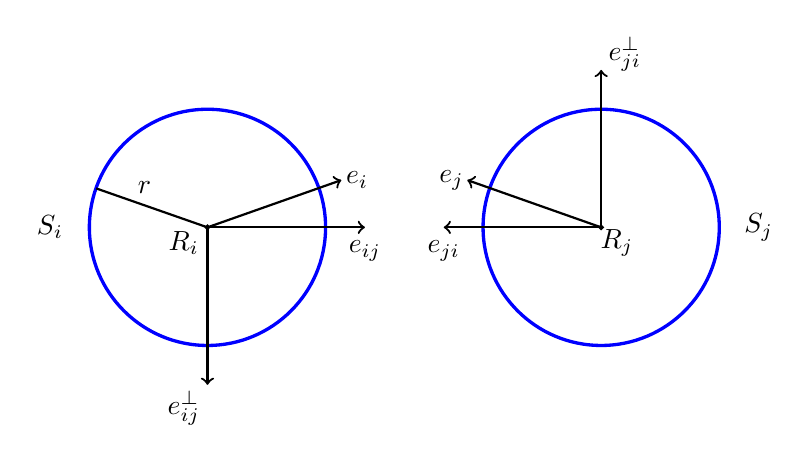
\begin{tikzpicture}
   
   \draw[color=blue, very thick](5,5) circle (1.5);
   \draw[color=blue, very thick](0,5) circle (1.5);
   
   \draw[color=black, very thick](0,5) circle (0.01);
   \draw[color=black, very thick](5,5) circle (0.01);
   
   \node  at (-0.3,5-0.2) {{$R_i$}};
   \node  at (5+0.2,5-0.2) {{$R_j$}};
   
   \node  at (-2,5) {{$S_i$}};
   \node  at (7,5) {{$S_j$}};
   
   \draw[thick, ->] (0,5) -- (1.7,5+0.6);
   \draw[thick, ->] (5,5) -- (5-1.7,5+0.6);
   
   \node  at (1.9,5+0.6) {{$e_i$}};
   \node  at (5-1.9,5+0.6) {{$e_j$}};
   
   \draw[thick] (0,5) -- ({-cos(45)*2}, {5+0.7*sin(45)});
   \node  at (-0.8,5+0.5) {{$r$}};
   
   \draw[thick, ->] (0,5) -- (2,5);
   \draw[thick, ->] (5,5) -- (3,5);
   
   \node  at (2,5-0.3) {{$e_{ij}$}};
   \node  at (3,5-0.3) {{$e_{ji}$}};
   
   \draw[thick, ->] (0,5) -- (0,3);
   \node  at (-0.3,3-0.3) {$e^{\perp}_{ij}$};
   
   
   \draw[thick, ->] (5,5) -- (5,7);
   \node  at (5+0.3,7+0.2) {$e^{\perp}_{ji}$};
   
   \end{tikzpicture}
   \end{center}
The figure shows the different vectors involved in the computations which will follow.
\\We define : 
\begin{itemize}
    \item $W_n(\mathrm{cos}(\theta))$ = $\frac{2}{n(n+1)}Pn'(\mathrm{cos}(\theta))$ \cite{Brumley}
    \item $P_n(\mathrm{cos}(\theta))$ the Legendre polynomials \cite{Wikipedia}
    \item $e_i.e_{ij} = \mathrm{cos}(\theta)$
    \item $e_i.e^{\perp}_{ij}$ = $\frac{(Y_{R_j} - Y_{R_i})\mathrm{cos}(\theta) - (X_{R_j} - X_{R_i})\mathrm{sin}(\theta)}{\lvert R_{ij} \rvert} $
\end{itemize}
\subsection{Forces}
The tangential lubrification forces acting on the two spheres can be calculated explicitly by :
\\ $F_z^{S_i}$ = $-9 \mu \pi r \frac{\lambda ^2}{(\lambda +1)^2} \sum_{n} \left[ B_n W_n(e_i.e_{ij})e_i.e_{ij} + \frac{1}{2} B_n W_n'(e_i.e_{ij})(e_i.e^{\perp}_{ij})^2 \right] (ln \epsilon + O(1))$ \cite{Brumley}

For $n$ = 1 : \begin{align*}
    W_1(\mathrm{cos}(\theta)) &= -\mathrm{sin}(\theta) \\
    W_1'(\mathrm{cos}(\theta)) &= -\mathrm{cos}(\theta) \\
    B_1 W_1(\mathrm{cos}(\theta))e_i.e_{ij}+ \frac{1}{2} B_1  W_1'(\mathrm{cos}(\theta)) (e_i.e^{\perp}_{ij})^2  &= -B_1 \mathrm{sin}(\theta)e_i.e_{ij} - \frac{1}{2} B_1  \mathrm{cos}(\theta) (e_i.e^{\perp}_{ij})^2 \\
    &= -B_1 \mathrm{sin}(\theta)\mathrm{cos}(\theta) - \frac{1}{2} B_1  \mathrm{cos}(\theta) (e_i.e^{\perp}_{ij})^2
\end{align*} 
For $n$ = 2 : \begin{align*}
    W_2(\mathrm{cos}(\theta)) &= -\mathrm{cos}(\theta)\mathrm{sin}(\theta) \\
    W_2'(\mathrm{cos}(\theta)) &= \mathrm{cos}^2(\theta)+ \mathrm{sin}^2(\theta) = 1\\
    B_2 W_2(\mathrm{cos}(\theta))e_i.e_{ij}+ \frac{1}{2} B_2  W_2'(\mathrm{cos}(\theta)) (e_i.e_x)^2  &= -B_2 \mathrm{cos}(\theta)e_i.e_{ij} - \frac{1}{2} B_2 (e_i.e^{\perp}_{ij})^2 \\
    &= -B_2 \mathrm{cos}^2(\theta) - \frac{1}{2} B_2 (e_i.e^{\perp}_{ij})^2
\end{align*}  

So :
\begin{equation*}
\footnotesize
\boxed{
    F_z^{S_i} = -9 \mu \pi r \frac{\lambda ^2}{(\lambda +1)^2} \left[ -B_1 \mathrm{sin}(\theta)\mathrm{cos}(\theta) - \frac{1}{2} B_1  \mathrm{cos}(\theta) (e_i.e^{\perp}_{ij})^2 -B_2 \mathrm{cos}^2(\theta) - \frac{1}{2} B_2 (e_i.e^{\perp}_{ij})^2(e_i.e^{\perp}_{ij})^2\right](ln \epsilon + O(1))}
\end{equation*}
\normalsize
\vspace{0.5cm}

The normal forces acting on the two spheres can be calculated explicitly by : \\
 $F_x^{S_i}$ = $-\frac{4}{5} \mu \pi r \frac{\lambda(\lambda +4)}{(\lambda +1)^2} \sum_{n} B_n W_n(e_i.e_{ij}) (ln \epsilon + O(1))$ \cite{Brumley}
\\ So :
\begin{equation*}
    \boxed{F_x^{S_i} = -\frac{4}{5} \mu \pi r \frac{\lambda(\lambda +4)}{(\lambda +1)^2} \left[ -B_1\mathrm{sin}(\theta) -B_2\mathrm{cos}(\theta)\mathrm{sin}(\theta)\right] (ln \epsilon + O(1))}
\end{equation*}

\subsection{The evolution of $\theta_i$}
The evolution of the rotation of one squirmer is given by : 
$$
\frac{d \theta_i}{dt} = \sum \Gamma_{ij->i} + \sum \Gamma_{ji->i} +  \Gamma_{i}^W.
$$

$\Gamma_{ij->k}$ the torque exerted on the $k^\mathrm{th}$ particle by the flow associated to the $i^\mathrm{th}$ particle, but perturbed by the presence of the $j^\mathrm{th}$ particle.\\

\vspace{0.5cm}

The torques in y axes acting on the squirmer $i$ can be calculated explicitly by : \\
$T_y^{S_i}$ = $\frac{16 \lambda}{5(\lambda +1)} \mu \pi r^2 e_i.e^{\perp}_{ij}\sum_{n} B_n W_n(e_i.e_{ij}) (ln \epsilon + O(1))$ \cite{Brumley}
\\ So :
\begin{equation*}
    \boxed{T_y^{S_i} = \frac{16 \lambda}{5(\lambda +1)} \mu \pi r^2 e_i.e^{\perp}_{ij}\left[-B_1\mathrm{sin}(\theta) -B_2\mathrm{cos}(\theta)\mathrm{sin}(\theta) \right] (ln \epsilon + O(1))}
\end{equation*}

The torques in y axes acting on the squirmer $j$ can be calculated explicitly by : \\
$T_y^{S_j}$ = $\frac{4 \lambda^2}{5(\lambda +1)} \mu \pi r^2 e_i.e^{\perp}_{ij}\sum_{n} B_n W_n(e_i.e_{ij}) (ln \epsilon + O(1))$ \cite{Brumley}
\\ So :
\begin{equation*}
    \boxed{T_y^{S_j} = \frac{4 \lambda^2}{5(\lambda +1)} \mu \pi r^2 e_i.e^{\perp}_{ij}\left[-B_1\mathrm{sin}(\theta) -B_2\mathrm{cos}(\theta)\mathrm{sin}(\theta) \right] (ln \epsilon + O(1))}
\end{equation*}

\newpage
\section{Implementation}
In this section we will detail the files of the \texttt{\href{https://github.com/master-csmi/2024-m1-nemo/tree/main/Code}{Code}} directory.

\subsection{codemat}
This file is the original matlab code that we re-implemented in Python.

\subsection{squirmer}
The first file contains the \texttt{Squirmer} class which takes the initial parameters: 
\begin{itemize}
   \item coordinates \texttt{x} and \texttt{y}
   \item \texttt{orientation}
   \item \texttt{radius}
   \item \texttt{beta}
   \item \texttt{velocity}
\end{itemize}
of a squirmer and compute \texttt{B1} and \texttt{B2}.

\subsection{csv\_file}
This file contains two function:
\begin{itemize}
   \item \texttt{export\_data\_csv(filename, data)} takes a file name and data from \texttt{loop\_time()} (section \texttt{interactingsquirmers}) and export it.
   \item \texttt{read\_csv\_file(filename)} takes a file name and return the data, not currently utilized but may be usefull for future functions.
\end{itemize}

\subsection{interactingsquirmers}
\subsubsection*{Parameters}
This file implements the \texttt{Interactingsquirmers} class which takes:
\begin{itemize}
   \item two \texttt{Squirmer}
   \item \texttt{R}, half of the length of one side of the square in which the two \texttt{Squirmer} will move
   \item \texttt{dt}, the time step and \texttt{dt\_out} the time step for output
   \item \texttt{T}, the final time of simulation
   \item \texttt{Es}, the amplitude (intensity) of steric interactions
   \item \texttt{ds}, the distance where the steric interactions become significative
   \item \texttt{mu}, the viscosity
   \item \texttt{Eo}, the amplitude of lubrication torque interactions
   \item \texttt{lnEps\_cr}, threshold value for \( -\log(\epsilon) \)
\end{itemize}

\subsubsection*{Methods}
This class has many functions:
\begin{itemize}
   \item \texttt{is\_in\_square()} and \texttt{check\_squirmers\_square()} verify if the $Squirmers$ 
   in argument are initially in the square.
   \item \texttt{distance\_sq()} return $(Dx, Dy)$ the directional vector of $R_{i}$ to $R_{j}$ 
   and the distance between the two.
   \item \texttt{forcesSteric(Dx, Dy, dist)} return the steric forces $(Fs_x, Fs_y)$ computed with the directional vector and the distance calculated with \texttt{distance\_sq()}.
   \item \texttt{forcesLubrification()} and \texttt{torquesLubrification()} each accept an argument $choice$ (1 for squirmer1 and 2 for squirmer2)
   and return the according lubrification forces and torques.
   \item \texttt{loop\_time()} is the primary function which update the positions and orientations of each $Squirmer$
   for each time step \texttt{dt} based on the lubrification forces and torques computed by \texttt{forcesLubrification()}, 
   \texttt{torquesLubrification()} and \texttt{forcesSteric()}, then puts all of the relevant information in a list
   at each time step \texttt{dt\_out}. The function then returns the list.
   \item \texttt{plot\_squirmers\_position(history, filename, dir)} and \texttt{plot\_dist\_sq(history, filename, dir)} 
   each take the list of \texttt{loop\_time}, a file name and a directory name
   they then respectively plot the position of the $Squirmers$ and the distance between them over time.
   \item \texttt{run()} take three file name as inputs, for the csv file, position graph and distance graph name, 
   then execute \texttt{check\_squirmers\_square()} and \texttt{loop\_time()},
   export the data into a csv file in the \texttt{csv\_files} directory with \texttt{export\_data\_csv(filename\_csv, data)} 
   , then plot the positions and distances of the $Squirmers$ in the \texttt{graphs} with \texttt{plot\_squirmers\_position(history, filename\_pos, dir)}
   and \texttt{plot\_dist\_sq(history, filename\_dist, dir)}.
\end{itemize}

\section{Numerical experiments}
\subsection{Simulation of two squirmers interacting}
For the first simulation, we consider two interacting squirmers.
\begin{center}
   Position and orientation of two squirmers.
   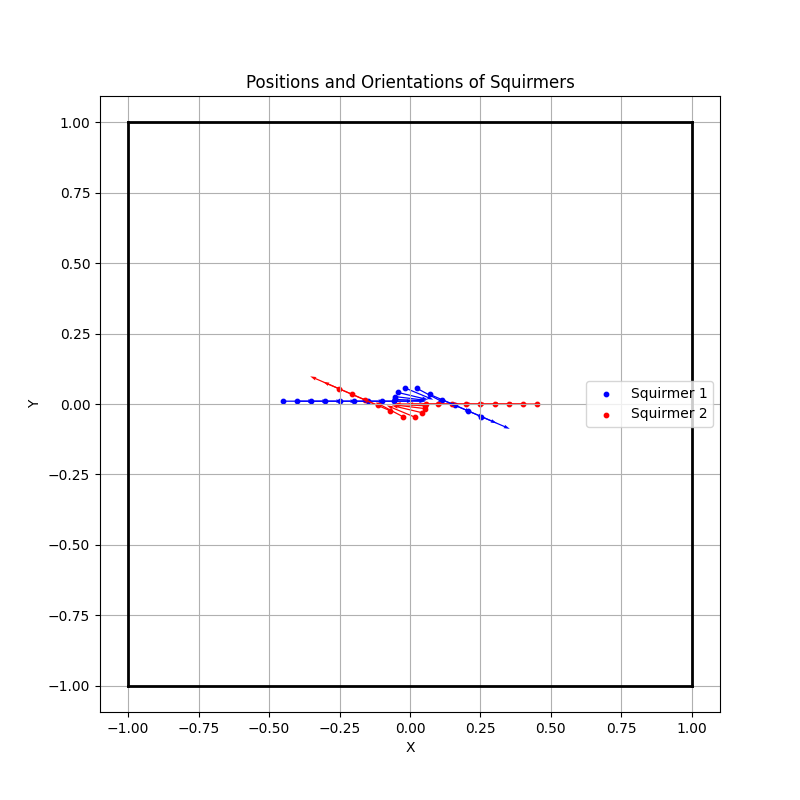
\includegraphics[width=0.7\textwidth]{graphs/squirmers_colliding.png}\\
   Distance between two squirmers
   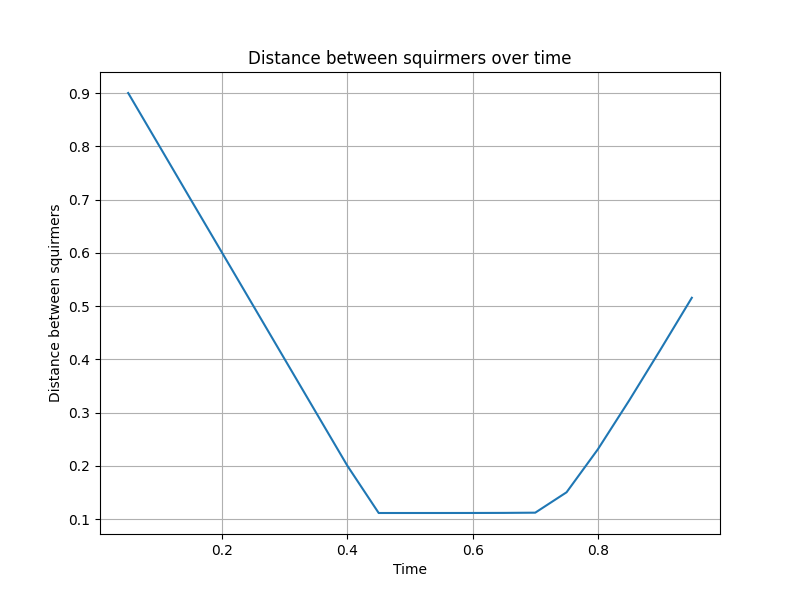
\includegraphics[width=0.7\textwidth]{graphs/dist_squirmers_colliding.png}
\end{center}
We show the trajectories of the two squirmers as well as their orientation. 
One can observe that their  orientation changes due to the lubrication and steric forces which are applied on them. 
This forces allow avoiding the overlapping of the two particles.
\newpage

\nocite{*}
\bibliographystyle{plain}
\bibliography{/bibliography/biblio}
\end{document}